 \documentclass [12pt]{article} 

\usepackage {amsmath}
\usepackage {amsthm}
\usepackage {amssymb}
\usepackage {graphicx} 
\usepackage {float}
\usepackage {multirow}
\usepackage {xcolor}
\usepackage {algorithmic}
\usepackage [ruled,vlined,commentsnumbered,titlenotnumbered]{algorithm2e} \usepackage {array} 
\usepackage {booktabs} 
\usepackage {url} 
\usepackage {parskip} 
\usepackage [margin=1in]{geometry} 
\usepackage [T1]{fontenc} 
\usepackage {cmbright} 
\usepackage [many]{tcolorbox} 
\usepackage [colorlinks = true,
            linkcolor = blue,
            urlcolor  = blue,
            citecolor = blue,
            anchorcolor = blue]{hyperref} 
\usepackage {enumitem} 
\usepackage {xparse} 
\usepackage {verbatim}
\usepackage{listings}
\usepackage{xcolor}
\lstset { %
    language=C++,
    backgroundcolor=\color{black!5}, % set backgroundcolor
    basicstyle=\footnotesize,% basic font setting
}
\newtheorem{theorem}{Theorem}
\newtheorem{remark}{Remark}



\DeclareTColorBox {Solution}{}{breakable, title={Solution}} \DeclareTColorBox {Solution*}{}{breakable, title={Solution (provided)}} \DeclareTColorBox {Instruction}{}{boxrule=0pt, boxsep=0pt, left=0.5em, right=0.5em, top=0.5em, bottom=0.5em, arc=0pt, toprule=1pt, bottomrule=1pt} \DeclareDocumentCommand {\Expecting }{+m}{\textbf {[We are expecting:} #1\textbf {]}} \DeclareDocumentCommand {\Points }{m}{\textbf {(#1 pt.)}} 

\begin {document} 

\vspace {1em} 
\begin {Instruction} 
Adapted From Virginia Williams' lecture notes.
\end {Instruction}  

{\LARGE \textbf {COMP 285 (NC A\&T, Spr `22)}\hfill \textbf {Lecture 13} } 

\begin{centering}
\section*{Hashing}
\end{centering}

\section{Hash tables}
A hash table is a commonly used data structure to store an unordered set of items, allowing constant time inserts, lookups and deletes (in expectation). Every item consists of a unique identifier called a key and a piece of information. For example, the key might be a Social Security Number, a driver's license number, or an employee ID number. The way in which a hash table stores a item depends only on its key, so we will only focus on the key here, but keep in mind that each key is usually associated with additional information that is also stored in the hash table.

A hash table supports the following operations:
\begin{itemize}
  \item Insert($k$): Insert key $k$ into the hash table.
  \item Lookup($k$): Check if key $k$ is present in the table.
  \item Delete($k$): Delete the key $k$ from the table.
\end{itemize}
Each operation will take constant time (in expectation).

\subsection{Implementation}
Let $U$ be the universe of all keys. For example, $U$ could be the set of all 64 bit strings. In this case $|U| = 2^64$. This is a very large universe, but we do not need to store all of these $2^64$ keys, we only need to store a subset $S \subset U$. Suppose that we know that the size of the subset we will need to store is less than or equal to $n$, which is much less than the size of the universe $|U|$. In a hash table of size $n$, each key  $k \in U$ is mapped to one of n ``buckets'' by a hash function $h : U \to \{1, 2, \cdots , n\}$. Since the universe $U$ is much larger than $n$, multiple
keys could map to the same hash bucket. To accommodate this, each bucket contains a linked list of keys currently stored in that bucket.

\textbf{Example}

Suppose we have a hash table of size $n = 5$ with hash function $h(x) = 13x + 2 \mod 5$. After inserting the elements $\{1, 2, 4, 7, 8\}$ the hash table looks like this:

\begin{center}
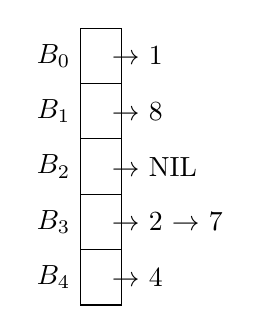
\begin{tikzpicture}
\coordinate (0);
\foreach \t[count=\i from 0,evaluate=\i as\j using int(\i+1)] in {
  1  ,
  8  ,
  NIL  ,
  2 $\rightarrow$ 7,
  4
}
\node at(\i.south)[anchor=north,draw,minimum height=2em,minimum width=1.5em,outer sep=0pt](\j){}
    node at(\j.west)[align=right,left]{$B_{\i}$} 
    node at(\j.east)[align=left,right,xshift=-.7em]{$\rightarrow$ \t};
\end{tikzpicture}
\end{center}

Where arrows denote pointers in the linked lists, and $B_2$ is empty. For example, $1$ is placed into bucket $B_0$ because $h(1) = 15 mod 5 = 0$.

\textbf{Time Complexity} 
ith this setup, the time required to perform an Insert, Lookup, or Delete operation on key $k$ is linear in the length of the linked list for the bucket that key $k$ maps to. We just use the hash function to find the correct bucket for an input key k, and then search the corresponding linked list for the element, inserting or deleting if necessary. Note that an Insert could be performed in constant time by always inserting at the head of the list, but we first need to check if key $k$ is already present.

\textbf{Choice of size of hash table} 
The hash table size is usually chosen so that the size of the hash table is at least as large as the maximum number of keys we will need to store at any point of time. If this condition is violated and the number of keys stored grows much larger than the size of the hash table, an implementation will usually increase the size of the table, and recompute the new table from scratch by mapping all keys to the bigger table. Our analysis ignores these complications and assumes that the number of keys is at most the hash table size.

\textbf{Potential problem with this implementation} 
In order for the operations to be implemented efficiently, we would like the keys to be distributed uniformly amongst the buckets in the hash table. We might hope that all buckets have at most a constant number of keys mapped to them, so that all operations could be performed in constant time. But for any fixed choice hash function $h$, one can always produce a subset of keys $S$ such that all keys in $S$ are mapped to the same location in the hash table. In this case, the running times of all operations will be linear in the number of keys - far from the constant we were hoping for. Thus, for a fixed hash function $h$, it is impossible to give worst case guarantees for the running times of hash table operations.

\textbf{Possible Solutions} 
There are two styles of analysis that we could use to circumvent this problem: 

\begin{enumerate}
  \item Assume that the set of keys stored in the hash table is random, or 
  \item Assume that the hash function $h$ is random. 
\end{enumerate}

Both are plausible alternatives. The problem with the first alternative is that it is hard to justify that the set of keys stored in the hash table is truly random. It would be more satisfying to have an analysis that works for any subset of keys currently in the hash table. In these notes, we will explore the second alternative, i.e., assume that the hash function $h$ is random.

































\end{document}

